\section{System Walkthrough}
\label{sec:walkthrough}
\subsection{From Instructor Setup to Student Access}
Figure~\ref{fig:lifecycle} follows one course through the application. After
sign-in, the user's role determines the workspace. An instructor configures a course they own through an
onboarding session. The session collects the tutoring policy,
source permissions and teaching settings. Uploaded PDF, text and Markdown
materials enter the reviewed ingestion workflow; parsing a document does not
itself authorize its use in student responses.

A release binds the reviewed policy, source versions, component profile and
applicable teaching-profile reference. Preflight checks readiness; publication
rechecks authority. Figure~\ref{fig:lifecycle} shows this distinction: revising
a draft does not change the release used by students.

\begin{figure}[htbp]
\centering
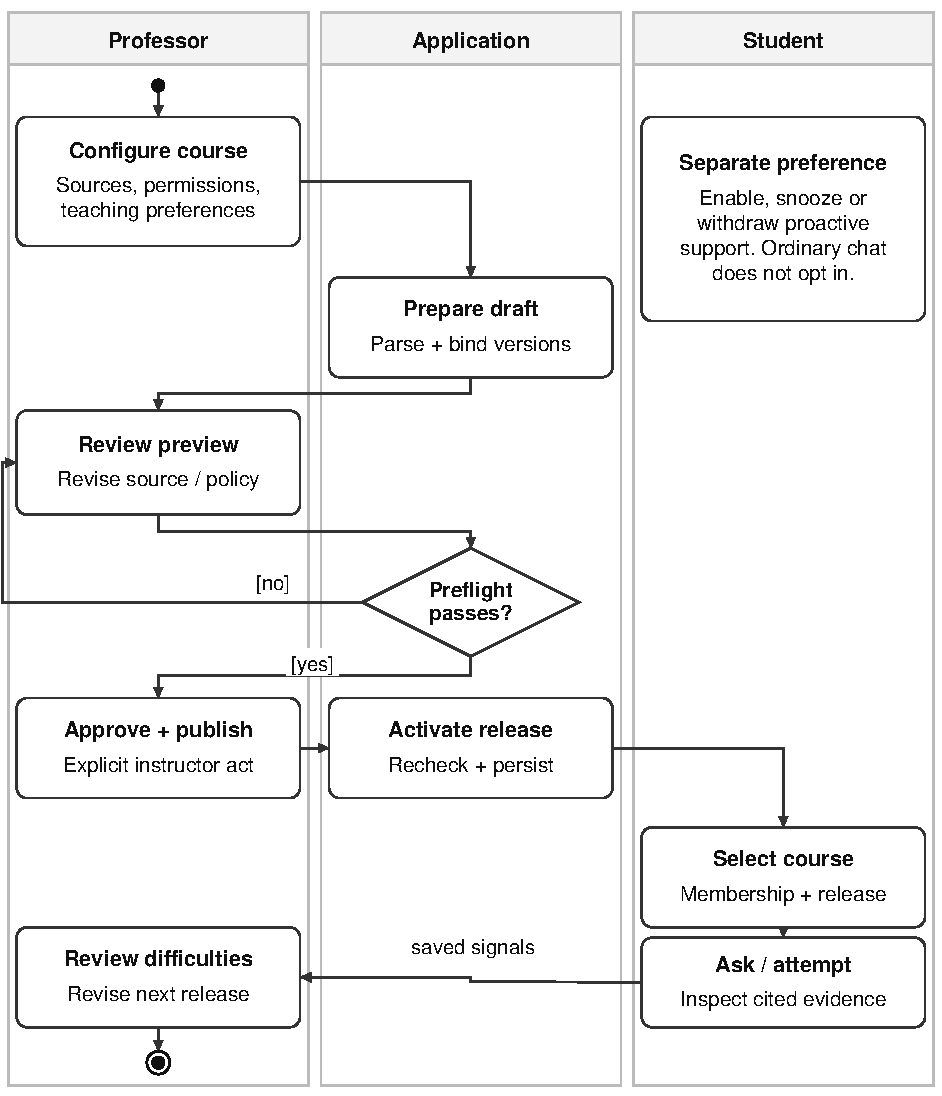
\includegraphics[width=\linewidth]{../../../reports/figures/course-twin-lifecycle.pdf}
\caption{One course configuration, publication and review cycle.}
\label{fig:lifecycle}
\end{figure}

Students select an available \emph{course}. Course membership and the published release determine which
Twin configuration the student can access. Opening a conversation associates its dialogue with that release.
A stored conversation is reused only when compatible with the current release;
withdrawn or incompatible contexts cannot authorize further tutoring.

The student asks a question, submits an attempt or opens a citation. Check-in
preferences are managed separately from ordinary chat. In the delivery workspace,
the professor can inspect goals, recorded action reasons and aggregate difficulty
signals, and pause autonomy or withdraw a release. The dashboard suppresses groups
with fewer than five learners. Its source-level difficulty summaries are signals
for instructor review, not diagnoses of individual understanding.

\subsection{From Configuration to Executable Behaviour}
The instructor's configuration has four layers (Table~\ref{tab:configuration}).
Structured action permissions restrict planning; descriptive teaching
preferences enter the configured generation pathway. The release-bound domain model maps
objectives to concepts and source evidence. Its diagnostic cues support concept
attribution, while the goal manager uses a fixed completion rule rather than
interpreting arbitrary success-condition prose.

\begin{table}[htbp]
\centering\small
\caption{Which part of the software consumes each instructor setting.}
\label{tab:configuration}
\begin{tabularx}{\linewidth}{@{}L{0.20\linewidth}Y Y@{}}
\toprule Setting & Runtime consumer & Observable effect and limit \\\midrule
Materials and permission & Ingestion, publication and retrieval & Restrict usable source versions and citation regions; upload alone does not authorize use. \\
Concepts and objectives & Attribution and goal lifecycle & Associate observed attempts with concepts; the corrected completion rule requires evidence for every concept of the exact objective. \\
Teaching preferences & Teaching-context and generation adapters & Supply tone, depth, examples and help sequence. The retained wording path is constrained; richer instruction is experimental. \\
Proactive policy & Event observer, planner and delivery service & Restrict actions and schedules; permit pause/stop. Timing, consent and frequency are checked separately from wording. \\
\bottomrule
\end{tabularx}
\end{table}

For example, the saved Socratic test profile requests a diagnostic question,
a student attempt and one hint. For the synthetic slot-seal question, its
actual first-turn response is: \emph{For \lq{}How does slot seal work\rq{}, what is
your current explanation, and which step are you unsure about?}
The response elicits an attempt but remains generic. The explanatory profile
permits a direct explanation; extracting a source rule alone does not establish
personalized progression. Appendix~\ref{sec:profile-examples} preserves the
eight-field synthetic configurations and actual response excerpts.

The instructor can also schedule support explicitly. The event-driven route
instead detects an opportunity from saved learner activity. Both routes can
reach the student without a new question. The following section explains how
observations, action selection and delivery connect, including where the
implemented connection remains approximate.
